\documentclass[10pt]{beamer}

\usetheme[progressbar=frametitle]{metropolis}
\usepackage{appendixnumberbeamer}

\usepackage{booktabs}
\usepackage[scale=2]{ccicons}

\usepackage{pgfplots}
\usepgfplotslibrary{dateplot}

\usepackage{xspace}
\newcommand{\themename}{\textbf{\textsc{metropolis}}\xspace}

\title{Chaos macht Schule - Datenschutz}
\subtitle{Schütz deine Daten, wenn du's nicht tust, tut's keiner!}
%TODO: Titel ist ja net grade schön
% "Datenschutz und Datensicherheit"?
% \date{\today}
\date{}
\author{Christoph Schindlbeck | Timo Schindler}
\institute{Binary Kitchen e.V.}
% \titlegraphic{\hfill\includegraphics[height=1.5cm]{logo.pdf}}

\begin{document}

\maketitle

\begin{frame}{Was passiert heute?}
  \setbeamertemplate{section in toc}[sections numbered]
  \tableofcontents[hideallsubsections]
\end{frame}

\section{Die Hacker, der CCC und die Kitchen}

%%%%%%%%%%%%%%%%%%%%%%%%%%%%%%%%%%%
%
% Crashkurs Hacker
%
%%%%%%%%%%%%%%%%%%%%%%%%%%%%%%%%%%%
\begin{frame}[fragile]{Crashkurs Hacker}

\begin{columns}[T,c,onlytextwidth]
\column{0.6\textwidth}
	\begin{figure}
		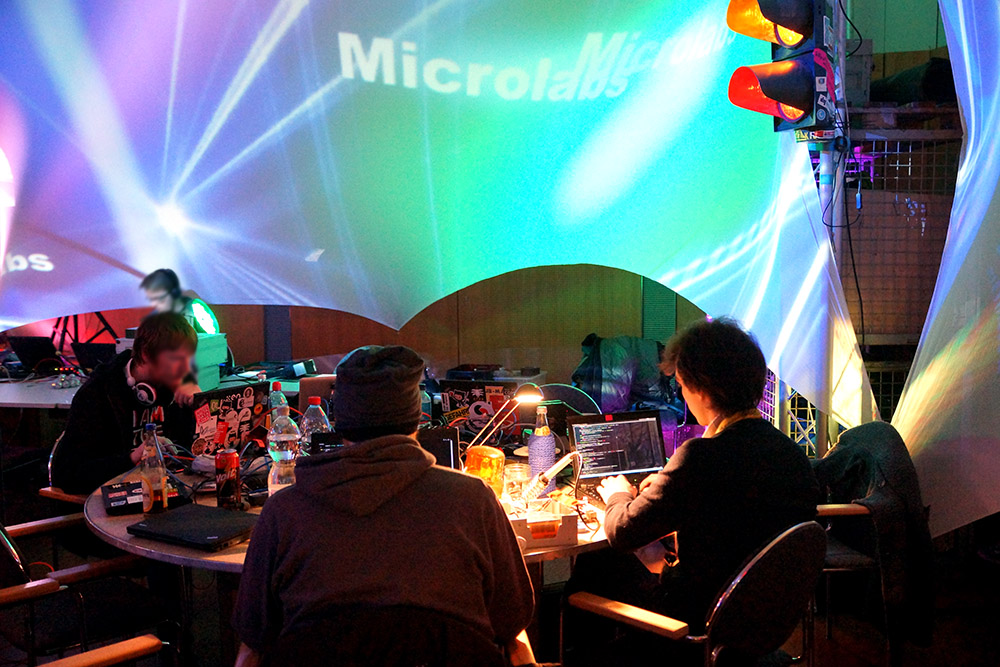
\includegraphics[width=1\textwidth]{images/DSC08058}
	\end{figure}

\column{0.4\textwidth}
\begin{itemize}
  	\item Skimaske !!11!
  	\item Beleuchtete Tastatur
  	\item Böse!
  	\item *hackhack* "I'm in!"
\end{itemize}
\end{columns}
\end{frame}

\begin{frame}[fragile]{Crashkurs Hacker}
	\begin{figure}
		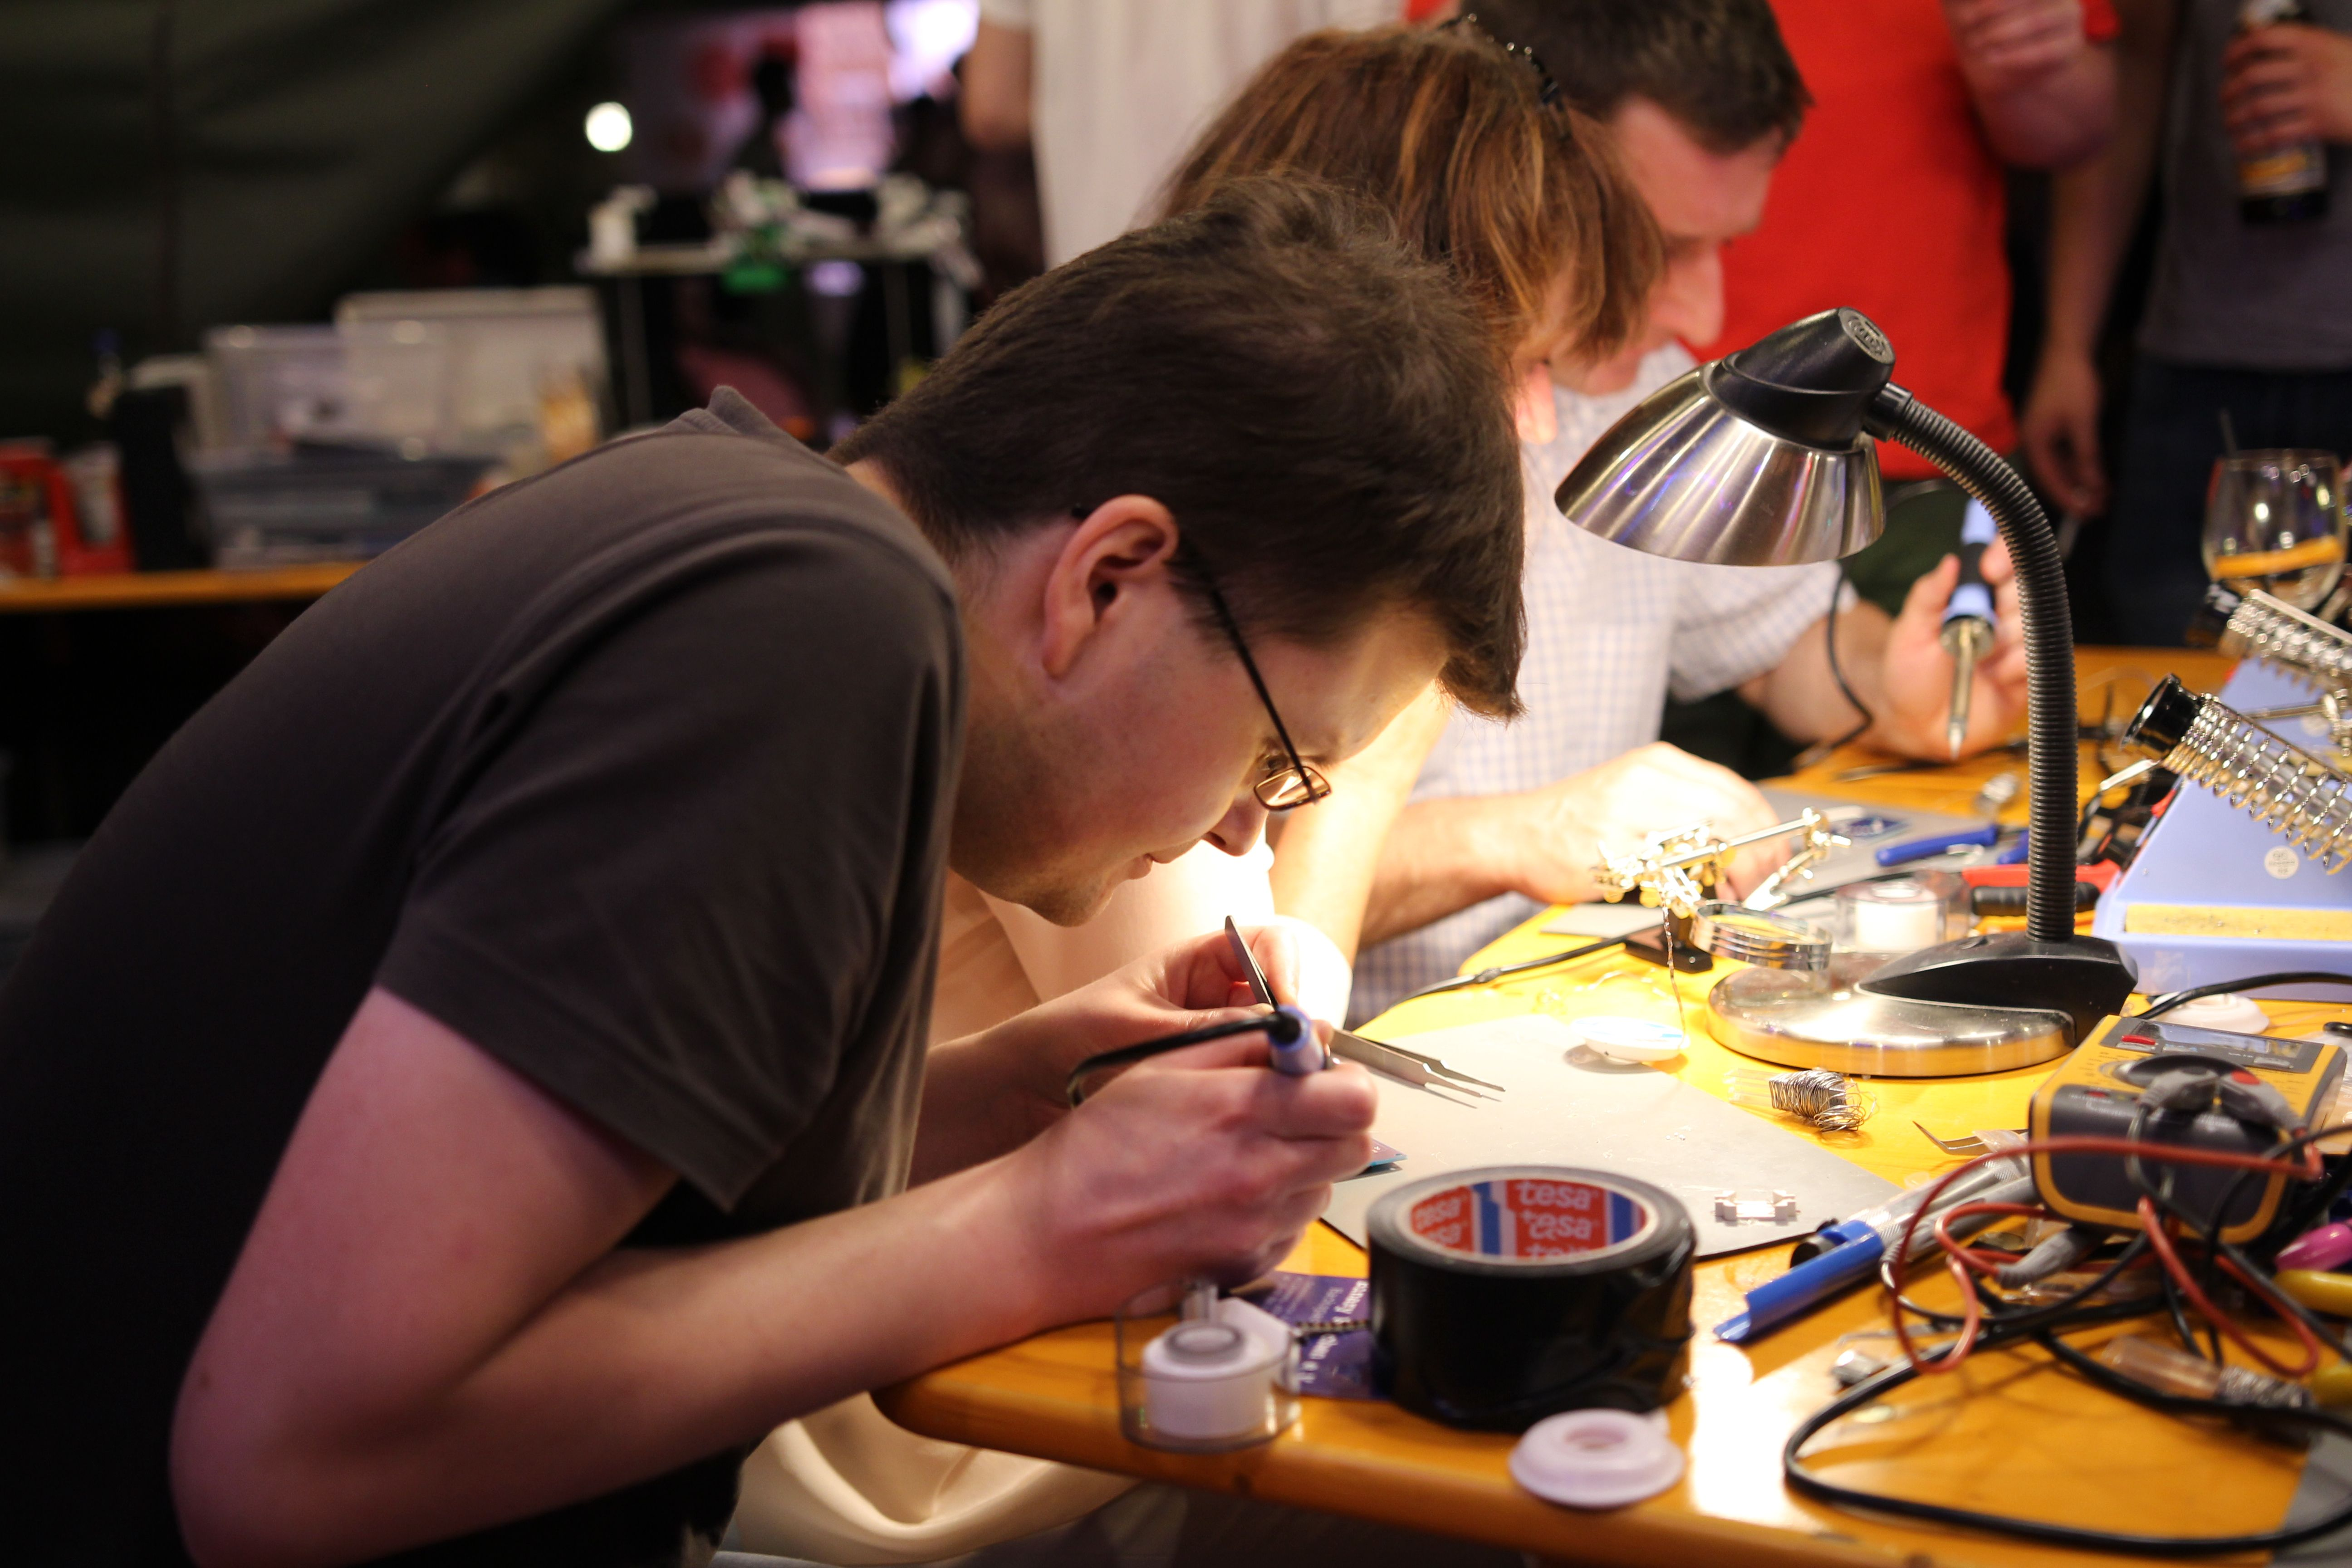
\includegraphics[width=1\textwidth]{images/IMG_6130}
	\end{figure}
\end{frame}

\begin{frame}[fragile]{Crashkurs Hacker}
	\begin{figure}
		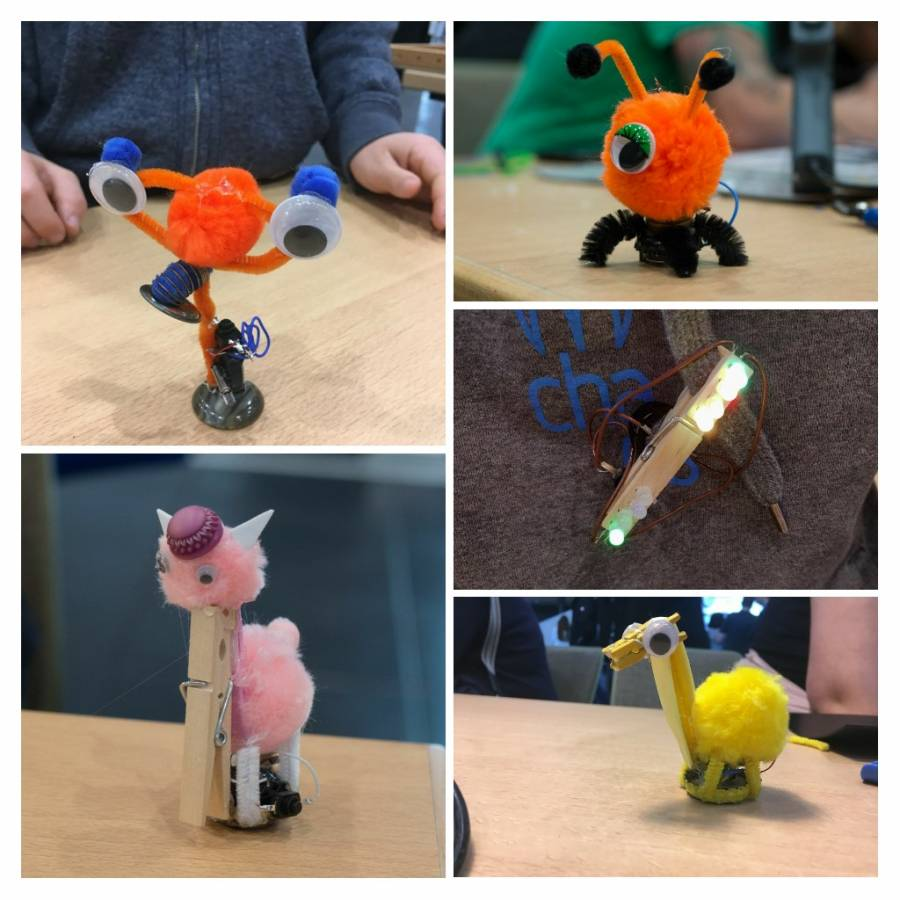
\includegraphics[width=.7\textwidth]{images/robots}
	\end{figure}
\end{frame}

%%%%%%%%%%%%%%%%%%%%%%%%%%%%%%%%%%%
%
% Der CCC
%
%%%%%%%%%%%%%%%%%%%%%%%%%%%%%%%%%%%
\begin{frame}[fragile]{Der CCC}
\begin{columns}[T,c,onlytextwidth]
\column{0.6\textwidth}
  \begin{itemize}
    \item Chaos Computer Club
    \item Gegründet 1981
    \item > 6000 Mitglieder
    \item Hackerethik
    \item Informationsfreiheit
    \item Auswirkungen von Technologien\\ auf die Gesellschaft
  \end{itemize}
\column{0.4\textwidth}
	\begin{figure}
		
\includegraphics[width=1\textwidth]{images/logo-ccc}
	\end{figure}
\end{columns}
\vspace{5mm}
\begin{center}
\alert{Private Daten schützen. Öffentliche Daten nützen.}
\end{center}
\end{frame}

%%%%%%%%%%%%%%%%%%%%%%%%%%%%%%%%%%%
%
% Die Binary Kitchen
%
%%%%%%%%%%%%%%%%%%%%%%%%%%%%%%%%%%%
\begin{frame}[fragile]{Die Binary Kitchen}
	\begin{figure}
		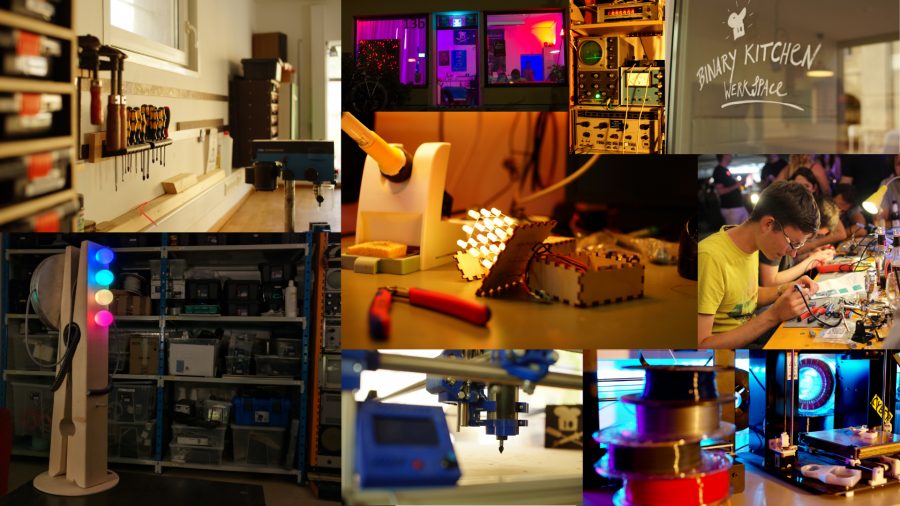
\includegraphics[width=1\textwidth]{images/bkcollage}
	\end{figure}

% Was erzählen?
%  \begin{itemize}
%    \item Binary Kitchen e.V.
%    \item Gemeinnütziger Verein
%    \item Hack- \& Makespace in Regensburg
%    \item Digitaler, sozialer und physischer Raum für Menschen
%    \item Nicht nur Technik!
%    \item Chaos macht Schule goes Regensburg
%  \end{itemize}

\end{frame}

\section{Datenschutzfails}

%%%%%%%%%%%%%%%%%%%%%%%%%%%%%%%%%%%
%
% Kündigung auf Twitter & Facebook
%
%%%%%%%%%%%%%%%%%%%%%%%%%%%%%%%%%%%
\begin{frame}[fragile]{Kündigung auf Twitter \& Facebook}
\begin{columns}[T,c,onlytextwidth]
\column{0.6\textwidth}
  \begin{itemize}
    \item Nutzer lästert über Arbeit
    \item ... Öffentlich
    \item Chef bekommt das mit
    \item Kündigung wird ausgestellt
    \item[] 
    \item[] 
    \item[] 
    \item[] 
  \end{itemize}
\column{0.4\textwidth}
	\begin{figure}
		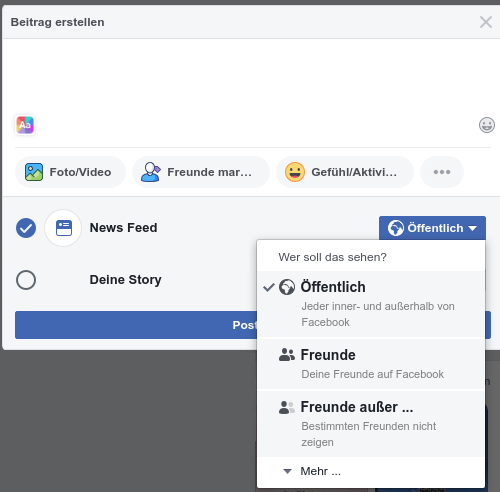
\includegraphics[width=1\textwidth]{images/facebook}
	\end{figure}
\end{columns}
% Quellen
% - https://anwalt-kg.de/newsbeitrag/arbeitsrecht/kuendigung-wegen-facebook-posts-die-gefahren-von-social-media/
% - https://www.spiegel.de/karriere/porsche-tweet-oder-facebook-post-als-kuendigungsgrund-a-1045323.html
% - https://www.express.de/news/politik-und-wirtschaft/recht/-morgen-faengt-mein-scheiss-job-an--frau-nach-frechem-tweet-gekuendigt---via-twitter-2787652
\end{frame}

\begin{frame}[fragile]{Kündigung via Twitter \& Facebook}
\begin{columns}[T,c,onlytextwidth]
\column{0.6\textwidth}
  \begin{itemize}
    \item Benutzer lästert über Arbeit
    \item ... Öffentlich
    \item Chef bekommt das mit
    \item Kündigung wird ausgestellt
    \item \alert{Pseudonym verwenden}
    \item \alert{Reichweite einschränken}
    \item \alert{Tweets/Posts wieder löschen}
    \item \alert{Überlegt euch was ihr postet}
  \end{itemize}
\column{0.4\textwidth}
	\begin{figure}
		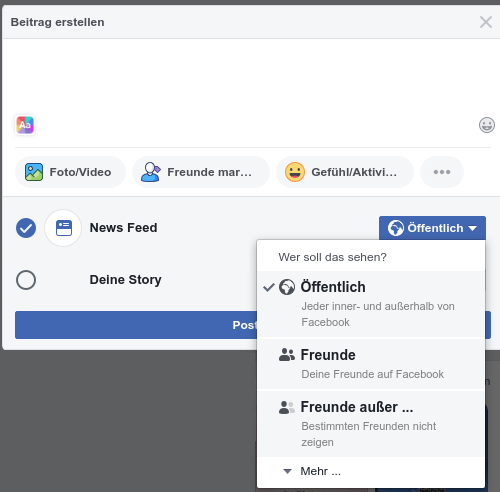
\includegraphics[width=1\textwidth]{images/facebook}
	\end{figure}
\end{columns}
% Quellen
% - https://anwalt-kg.de/newsbeitrag/arbeitsrecht/kuendigung-wegen-facebook-posts-die-gefahren-von-social-media/
% - https://www.spiegel.de/karriere/porsche-tweet-oder-facebook-post-als-kuendigungsgrund-a-1045323.html
% - https://www.express.de/news/politik-und-wirtschaft/recht/-morgen-faengt-mein-scheiss-job-an--frau-nach-frechem-tweet-gekuendigt---via-twitter-2787652
\end{frame}

%%%%%%%%%%%%%%%%%%%%%%%%%%%%%%%%%%%
%
% TODO: Zyklus-App abschnitt schreiben
%
%%%%%%%%%%%%%%%%%%%%%%%%%%%%%%%%%%%
\begin{frame}[fragile]{Zyklus-Apps}
\begin{itemize}
    \item Nützlich, um den weiblichen Zyklus zu überwachen
    
    \item Sehr sensible Daten, nicht nur über Verhütungsmaßnahmen
    \item Plötzlich Werbung für Babysachen auf Facebook
    
    %\item Mehrere große Apps haben diese Daten an Facebook weiter gegeben
    \item \alert{Achtet auf die Datenschutzeinstellungen!}
    \item \alert{Keine privaten Daten an fragwürdige Apps}
    \item Gibt es Offline-Alternativen?
\end{itemize}
% https://netzpolitik.org/2019/zyklus-apps-geben-intime-daten-an-facebook-weiter/
% Was passiert mit euren Daten?
% Warum muss das in die Cloud?
% Keiner weiß, was mit euren Daten weiter passiert
\end{frame}

%%%%%%%%%%%%%%%%%%%%%%%%%%%%%%%%%%%
%
% Facebook is watching you
%
%%%%%%%%%%%%%%%%%%%%%%%%%%%%%%%%%%%
\begin{frame}[fragile]{Facebook is watching you!}
\begin{itemize}
    \item Facebook-App aktiviert Frontkamera (12.11.19)
    \item Nicht sichtbar für Benutzer
    \item Was macht ihr gerade?
    \item Was passiert mit den Daten?
    \item[]
    \item[]
    \item[]
  \end{itemize}
% natürlich versehentlich
% https://www.n-tv.de/technik/Warum-nutzt-Facebook-heimlich-die-Kamera-article21390710.html
% TODO: Bessere Quelle
\end{frame}

\begin{frame}[fragile]{Facebook is watching you!}
\begin{itemize}
    \item Facebook-App aktiviert Frontkamera (12.11.19)
    \item Nicht sichtbar für Benutzer
    \item Was macht ihr gerade?
    \item Was passiert mit den Daten?
    \item \alert{Simpel: Kamera abkleben}
    \item \alert{Berechtigung einschränken}
    \item \alert{Viele weitere Sensoren}
  \end{itemize}
% natürlich versehentlich
% https://www.n-tv.de/technik/Warum-nutzt-Facebook-heimlich-die-Kamera-article21390710.html
% TODO: Bessere Quelle
% TODO: Bild?
\end{frame}

\begin{frame}[fragile]{Einreise verweigert wegen privater Nachrichten}
\begin{itemize}
    \item Schülerin spricht auf Facebook über Reise nach Amerika
    \item Soll auf Kinder aufpassen...
    \item ... und soll Geld dafür bekommen
    \item Einreise verweigert wegen illegaler Arbeit
    \item[]
    \item[]
    \item[]
    \item[]
  \end{itemize}
% https://www.spiegel.de/lebenundlernen/schule/usa-einreise-abgelehnt-20-jaehrige-wegen-facebook-chat-abgewiesen-a-1046792.html
% https://www.n-tv.de/technik/Warum-nutzt-Facebook-heimlich-die-Kamera-article21390710.html
% Auf sichere Kommunikation eingehen
%TODO: Foto einfügen?
\end{frame}

\begin{frame}[fragile]{Einreise verweigert wegen privater Nachrichten}
\begin{itemize}
    \item Schülerin spricht auf Facebook über Reise nach Amerika
    \item Soll auf Kinder aufpassen...
    \item ... und soll Geld dafür bekommen
    \item Einreise verweigert wegen illegaler Arbeit
    \item \alert{Reist nicht nach Amerika ;)}
    \item \alert{Wie kann Kommunikation ausgelegt werden?}
    \item \alert{Sichere Messenger verwenden!}
    \item \alert{Cloud Act}
  \end{itemize}
% https://www.spiegel.de/lebenundlernen/schule/usa-einreise-abgelehnt-20-jaehrige-wegen-facebook-chat-abgewiesen-a-1046792.html
% https://www.n-tv.de/technik/Warum-nutzt-Facebook-heimlich-die-Kamera-article21390710.html
% Auf sichere Kommunikation eingehen
%TODO: Foto einfügen?
\end{frame}


\section{Datensicherheit}

%%%%%%%%%%%%%%%%%%%%%%%%%%%%%%%%%%%
%
% Die schnöden Metadaten
%
%%%%%%%%%%%%%%%%%%%%%%%%%%%%%%%%%%%
\begin{frame}[fragile]{Die schnöden Metadaten}
	\begin{figure}
		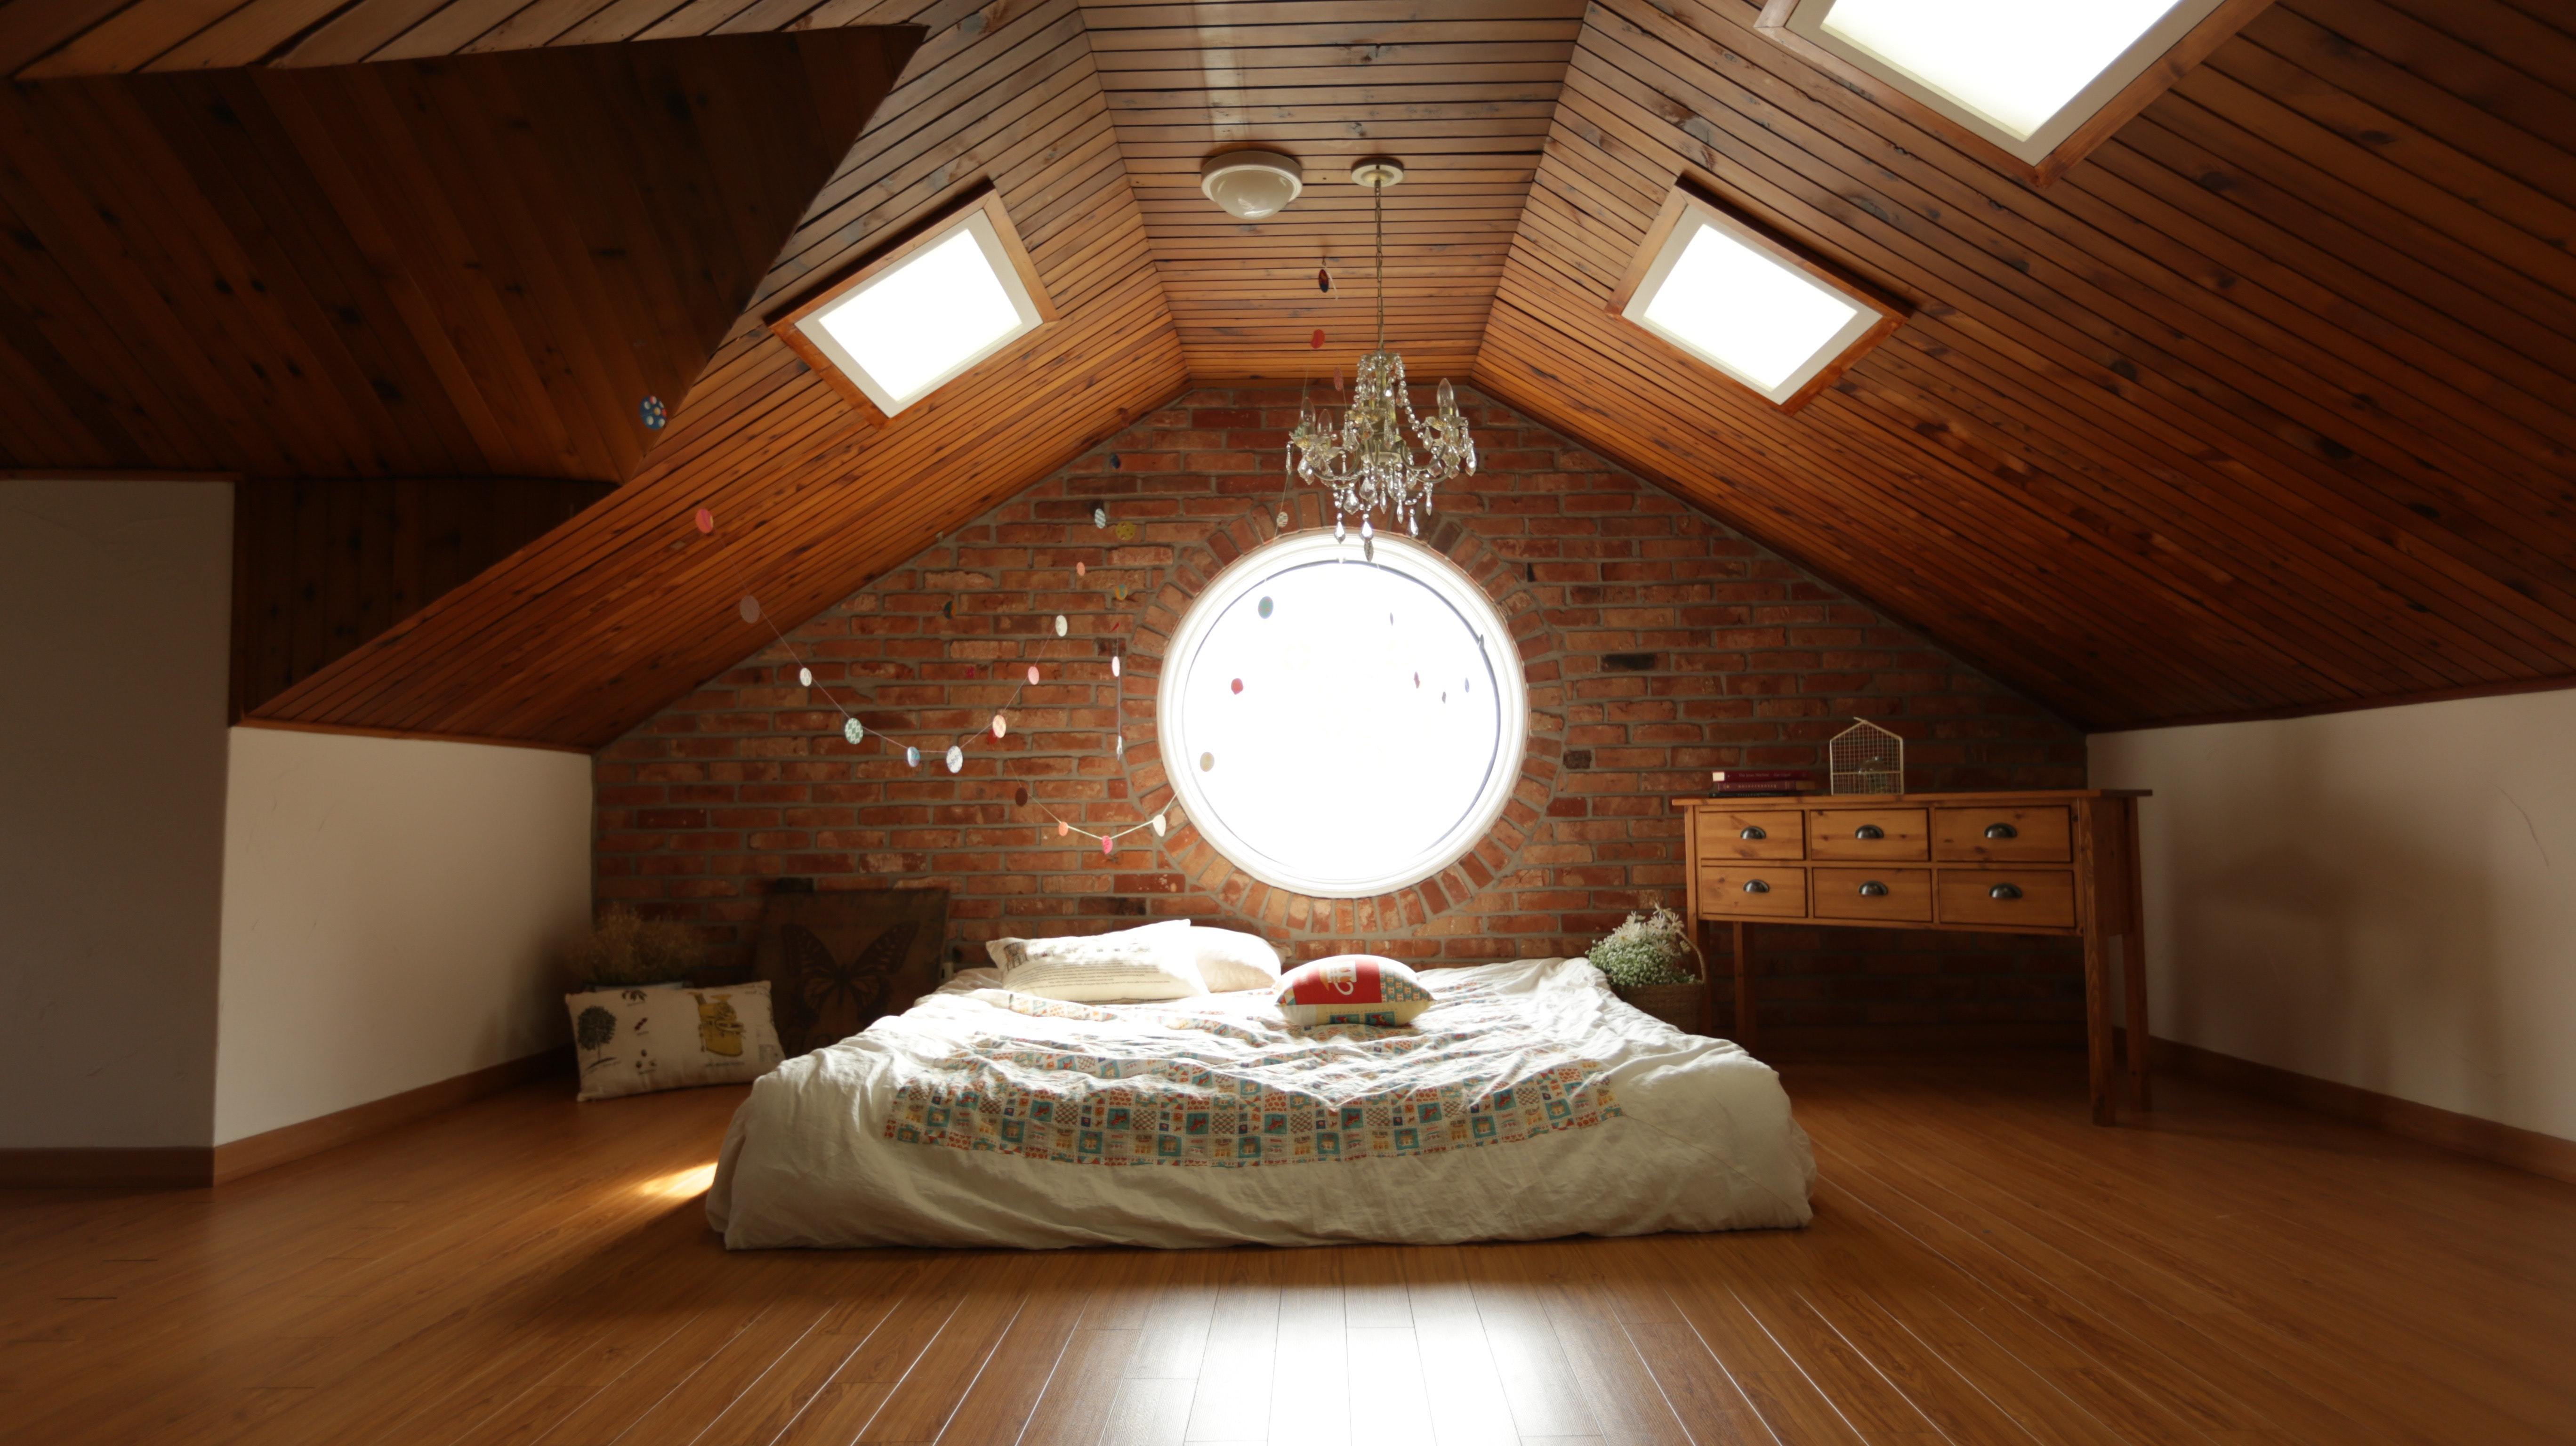
\includegraphics[width=1\textwidth]{images/CMS_Methodensammlung_Metadaten}
			\tiny Quelle: Pexels, CC0-Lizenz
	\end{figure}
% Was kann man durch die Metadtaten alles herausfinden?
% Vor allem auf Bilder eingehen
% Was kann aus Bildern extrahiert werden?
% Spiegel-online Mining!
\end{frame}

\begin{frame}[fragile]{Die schnöden Metadaten}
\begin{columns}[T,c,onlytextwidth]
\column{0.5\textwidth}
	\begin{figure}
		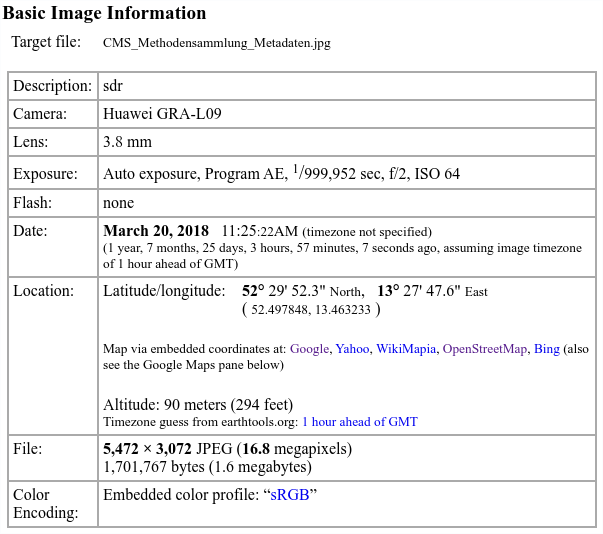
\includegraphics[width=1\textwidth]{images/meta1}
		\tiny Quelle: exif.regex.info \& openstreetmap.org
	\end{figure}
\column{0.5\textwidth}
	\begin{figure}
		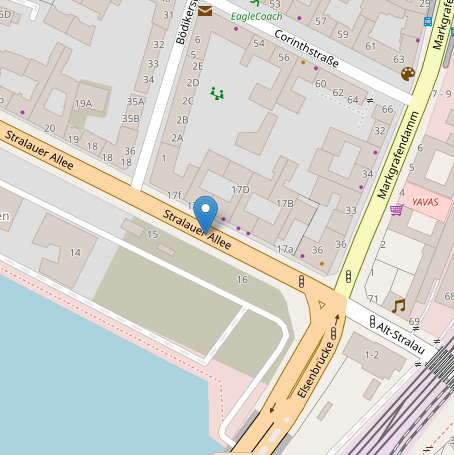
\includegraphics[width=1\textwidth]{images/meta2}
	\end{figure}
\end{columns}

% Was kann man durch die Metadtaten alles herausfinden?
% Vor allem auf Bilder eingehen
% Was kann aus Bildern extrahiert werden?
% Spiegel-online Mining!
\end{frame}

%%%%%%%%%%%%%%%%%%%%%%%%%%%%%%%%%%%
%
% Sicheres P422wORt?
%
%%%%%%%%%%%%%%%%%%%%%%%%%%%%%%%%%%%
\begin{frame}[fragile]{Sicheres P422wORt?}
\begin{itemize}
    \item Size matters!
    \item Länge wichtiger als Komplexität
    \item "abcdefghi" (9 Buchstaben) -> \alert{5 Tage}
    \item "abcdefghijk" (11 Buchstaben) -> \alert{10 Jahre}
    \item Niemals gleiche Passwörter
    \item \alert{Passwortmanager}
    \item \alert{Emailpassword unendlich wichtig}
    \item \alert{Zweiter Faktor}
    \item \alert{https://haveibeenpwned.com/ - have i been pwned?}
  \end{itemize}
\end{frame}

\section{Gesammelte Daten und was damit passieren kann}

%%%%%%%%%%%%%%%%%%%%%%%%%%%%%%%%%%%
%
% Emotet, König der Schadsoftware
%
%%%%%%%%%%%%%%%%%%%%%%%%%%%%%%%%%%%
\begin{frame}[fragile]{Emotet, König der Schadsoftware}
\begin{itemize}
    \item Perfides Mistding
    \item Täuschend echte Emails
    \item Späht Email-Konto aus
    \item Vielseitig nachladbar
    \item Email-Adresse zentraler Dreh- und Angelpunkt
  \end{itemize}
\end{frame}

%%%%%%%%%%%%%%%%%%%%%%%%%%%%%%%%%%%
%
% Werbung als Einfallstor und Tracker
%
%%%%%%%%%%%%%%%%%%%%%%%%%%%%%%%%%%%
\begin{frame}[fragile]{Werbung als Einfallstor und Tracker}
\begin{columns}[T,c,onlytextwidth]
\column{0.6\textwidth}
\begin{itemize}
    \item Werbung nervt. Jeden.
    \item Werbung trackt
    \item Werbung gefährdet
    \item Werbung kostet traffic
    \item \alert{Werbeblocker nutzen}
  \end{itemize}
\column{0.4\textwidth}
	\begin{figure}
		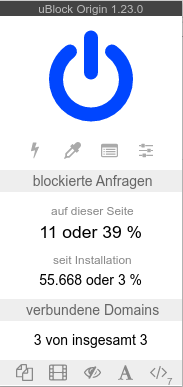
\includegraphics[width=.7\textwidth]{images/ublock}
	\end{figure}
\end{columns}
\end{frame}

%%%%%%%%%%%%%%%%%%%%%%%%%%%%%%%%%%%
%
% Werbung als Einfallstor und Tracker
%
%%%%%%%%%%%%%%%%%%%%%%%%%%%%%%%%%%%
\begin{frame}[fragile]{Google sammelt Gesundheitsdaten}
      \begin{alertblock}{Im "Project Nightingale" sammelt Google Gesundheitsdaten von Millionen Patienten in den USA. (14.11.2019)}
    \begin{itemize}
    \item Was passiert mit den Gesundheitsdaten?
    \item Einmal gesammelt, schnell in anderen Händen
    \item Stichwort: Rosa Listen
    \item Vision: Kein Kredit? Keine Krankenkasse?
  \end{itemize}
      \end{alertblock}
      \tiny Quelle: https://www.sueddeutsche.de/wirtschaft/patientendaten-ungesunde-naehe-1.4680297
% Was passiert mit den Daten?
% Thema Big Data
% Man weiß nicht, was passiert wenn die daten mal an andere gehen?
% Einmal gesammelte Daten bleiben (vgl. Rosa listen https://de.wikipedia.org/wiki/Rosa_Liste )
\end{frame}

%%%%%%%%%%%%%%%%%%%%%%%%%%%%%%%%%%%
%
% Welcher Schutz ist sinnvoll?
%
%%%%%%%%%%%%%%%%%%%%%%%%%%%%%%%%%%%
\begin{frame}[fragile]{Welcher Schutz ist sinnvoll?}
    \begin{itemize}
    \item Nachdenken
    \item Schützt euch mit Technik
    \item \alert{uBlock origin}
    \item \alert{KeePass}
    \item \alert{lastpass.com}
  \end{itemize}
% Browser Apps: https://www.klicksafe.de/fileadmin/media/documents/pdf/klicksafe_Materialien/Lehrer_Allgemein/ks_to_go_Datensatz_-_Datenschatz.pdf
\end{frame}

\section{Wie gehts weiter?}

%%%%%%%%%%%%%%%%%%%%%%%%%%%%%%%%%%%
%
% Weitere Infos
%
%%%%%%%%%%%%%%%%%%%%%%%%%%%%%%%%%%%
\begin{frame}{Weitere Infos}
\begin{itemize}
    \item Löchert uns mit Fragen!
    \item Besucht euren lokalen Hackspace
    \item Besucht eine Crypto-Party
    \item \alert{klicksafe.de/materialien}
  \end{itemize}
\end{frame}

%%%%%%%%%%%%%%%%%%%%%%%%%%%%%%%%%%%
%
% Fragen?
%
%%%%%%%%%%%%%%%%%%%%%%%%%%%%%%%%%%%
{\setbeamercolor{palette primary}{fg=black, bg=white}
\begin{frame}[standout]
  Fragen?
  	\begin{figure}
		
\includegraphics[width=.3\textwidth]{images/qrcode}
	\end{figure}
  \tiny https://github.com/Binary-Kitchen/chaos-macht-schule
  
  Präsentation:
  \ccbysa
\end{frame}
}

\end{document}
